
\section{Curl closure and duon current}\label{sec:curl-closure-duon-current}

\subsection{Curl forms}\label{subsec:curl-closure}
\subsubsection{Curl}\label{subsec:curl}
\begin{definition}[Curl. \appref{app:cc-curl}]
Curl is the Stokes-aligned circulation/closure object on the cited support. A\(\Omega\)D calculates its hinge return, reclosure, duration, orientation, and returned current on declared windows.
\end{definition}

\subsubsection{Nested curl}\label{subsec:nested-curl}
\begin{definition}[Nested curl. \appref{app:cc-nested-curl}]
A nested curl is a curl carried inside another curl.
\end{definition}

\subsubsection{Pin-curl}\label{subsec:pin-curl}
\begin{definition}[Pin-curl. \appref{app:cc-pin-curl}]
A pin-curl is a returned curl whose residue seats, delays, or fixes a hinge.
\end{definition}

\subsubsection{Curling curls}\label{subsec:curling-curls}
\begin{definition}[Curling curls. \appref{app:cc-curling-curls}]
Curling curls are recursive returns that become active path structure inside the fractal tesseract topology.
\end{definition}

\subsection{Monon beat}\label{subsec:monon-beat}
\begin{definition}[Monon. \appref{app:cc-monon}]
A monon is the primitive completed branch/hinge/branch cycle of \(x\succ x=x\). With local hinge triad
\[
\mathsf H_3(x)=(x^-,\mu,x^+),
\]
the monon cycle is written
\[
\mathrm{monon}(x)=\operatorname{cycle}_{\mathsf H_3}(x\succ x=x).
\]
The unindexed form \(\operatorname{cycle}(x\succ x=x)\) is the same primitive cycle when the hinge support is already fixed by context.
\end{definition}

\subsection{Dion}\label{subsec:dion}
\begin{definition}[Dion. \appref{app:cc-dion}]
A dion is the first two-position return curl around the monon hinge:
\[
D_\alpha=(+1,-1),\qquad D_\Omega=(-1,+1).
\]
\end{definition}

\subsection{Duon}\label{subsec:duon}
\begin{definition}[Duon. \appref{app:cc-duon-duad-cycle}]
A duon is Dion--hinge--Dion returned-current support. A compact unresolved form is
\[
\mathrm{duon}=D_i\Box D_j,
\qquad D_i,D_j\in\{D_\alpha,D_\Omega\}.
\]
A resolved duon carries the monon hinge / pivot value:
\begin{equation}
D_i\mu D_j,
\qquad
D_i,D_j\in\{D_\alpha,D_\Omega\},
\qquad
\mu\in\{-1,0,+1\}.
\label{eq:duon-current}
\end{equation}
\end{definition}

\subsubsection{Current cell}\label{subsec:duon-current-cell}
A duon current is carried hinge-current through cycle support. The primitive resolved family has
\[
2\times3\times2=12
\]
variants. Duon, duad, and temporal cycle presentation. \appref{app:cc-duon-duad-cycle}.

\subsubsection{Tick/click}\label{subsec:duon-tick-click}
Let \(K_t\) be a field cycle state. A tick emits a duon current
\[
X_t=E(K_t).
\]
A click receives a returned duon \(Y_t\). The cycle update is
\[
K_{t+1}=U(K_t,Y_t,\beta_t,\Delta_{\mathrm{lead/lag}}),
\]
and the next tick emits
\[
X_{t+1}=E(K_{t+1}).
\]

\subsubsection{Markovian and retained-history continuity}\label{subsec:duon-continuity}
A Markovian continuity continues by present cycle state. A retained-history continuity carries prior return, lead--lag burden, jitter, shell residue, duration, or SADAR channel memory. Both forms carry wave continuity when distinction-information persists through recurring duon cycle form.

\subsubsection{Branch/hinge/branch reflection duration}\label{subsec:branch-hinge-rd}
Reflection duration is counted on branch/hinge/branch return support. For a returned-current path history \(\gamma\) on \(B\),
\begin{equation}
RD_\gamma(B)
=
\Pi^-_\gamma(B)
+
H_{\mu,\gamma}(B)
+
\Pi^+_\gamma(B).
\label{eq:branch-hinge-rd}
\end{equation}
Here \(\Pi^-_\gamma\) is the first-branch support, \(H_{\mu,\gamma}\) is the hinge recurrence contribution, and \(\Pi^+_\gamma\) is the reflected return-branch support. If the branch supports are symmetric, \(\Pi^-_\gamma=\Pi^+_\gamma=\Pi\), then
\begin{equation}
RD_\gamma(B)=2\Pi+H_{\mu,\gamma}(B).
\label{eq:branch-hinge-rd-symmetric}
\end{equation}
The familiar \(RD=2\Pi+1\) is the single-hinge reduction \(H_{\mu,\gamma}=1\), not a universal hinge rule. For a retained cycle \(C\) on \(B\), write the reflection-duration accessor as
\[
RD_B(C)=\Pi^-_B(C)+H_{\mu,B}(C)+\Pi^+_B(C).
\]
RD is not coupling. RD is reflection duration.

\subsection{Duad}\label{subsec:duad}
\begin{definition}[Duad. \appref{app:cc-duon-duad-cycle}]
A duad is the seat-taken state of the same duon current.
\end{definition}

\subsection{Curling-curl support forms}\label{subsec:curling-curl-support-forms}

A compact expression \(p{:}q{:}L\) is a compressed curling-curl specification. The \(p{:}q\) part names the retained curling-curl support form, the construction trace admits it on \(B\), and \(L\) declares the enclosure/window support used by a downstream entry. In the single-hinge symmetric fixture,
\[
\Pi(p{:}q)=q^p+q,
\qquad
RD_B^{(1)}(p{:}q)=\Pi(p{:}q)+1+\Pi(p{:}q).
\]
Thus \(1{:}2\) gives \(\Pi=4\) and \(RD_B^{(1)}=9\); \(3{:}2\) gives \(\Pi=10\) and \(RD_B^{(1)}=21\); \(3{:}3\) gives \(\Pi=30\) and \(RD_B^{(1)}=61\); \(3{:}4\) gives \(\Pi=68\) and \(RD_B^{(1)}=137\). These are internal reflection-duration accessors of declared curling-curl specifications. The live calculus keeps the construction trace, isotropic/anisotropic Markov choice, hinge slide, jitter, boundary capacity, and admission status visible. Measured-sector interpretations, if any, belong to the manual external-comparison layer.

\begin{definition}[Support expression]
A support expression is formal syntax
\begin{equation}
\Sigma=(s_1,\ldots,s_m;L),
\label{eq:support-expression}
\end{equation}
where each \(s_i=p_i{:}q_i\) and \(L\) is an optional shared enclosure qualifier.
\end{definition}

\begin{definition}[Curling-curl support form]
A curling-curl support form is the retained recursive curl/cycle form proposed by a support expression and admitted on a declared boundary/window after its construction trace is declared or inherited.
\end{definition}

A compact expression such as \(1{:}2{:}6\), \(3{:}3{:}6\), or \(3{:}4{:}6\) proposes a specification \(K_{\mathrm{prop}}\). Admission is a traced calculation on the declared scope:
\begin{equation}
K_{\mathrm{prop}}
\xrightarrow{\,HT(K;B)\,}
K_{\mathrm{adm}}(B).
\label{eq:key-proposed-admitted-trace}
\end{equation}
Here \(HT(K;B)\) is the construction trace of the proposed specification on \(B\). The specification \(K_{\mathrm{prop}}\) does not by itself determine closure, pressure, shedding, or a measured-sector comparison label. Those are formed from the declared trace on \(B\).

The trace discipline is
\begin{equation}
\begin{aligned}
\Sigma/K_{\mathrm{prop}}
&\xrightarrow{\text{construction trace}}
HT(K;B)
\xrightarrow{\text{admission on }B}
K_{\mathrm{adm}}(B)\\
&\xrightarrow{\text{return-current trace}}
RD_h(B)
\xrightarrow{\bowtie_B R^{\mathrm{asym}}_h}
RCD_h(B)
\xrightarrow{\operatorname{dur}}
\rho_h^D(B)\\
&\xrightarrow{\min(\cdot,|\omega_h|)}
\rho^D_{\omega,h}(B)
\xrightarrow{C_{3,h}}
p_h^D
\xrightarrow{A_h}
\SADARop_B(C_h)
\xrightarrow{\text{closure test}}
\Delta_{\mathrm{close}}\\
&\xrightarrow{\max(0,\cdot)}
X_{\mathrm{shedding}}
\xrightarrow{\text{declared route}}
\operatorname{SheddicPath}.
\end{aligned}
\label{eq:support-trace-spine}
\end{equation}

The following are compact curling-curl specifications. Their admitted status, closure, hinge, pressure, and shedding are certified only by \(HT(K;B)\):
\[
1{:}2{:}6=\text{Dimonhexon}
=\text{Dimonon curling-curl support form carried on }C_6,
\]
with nesting, hinge, and closure details supplied by \(HT(1{:}2{:}6;B)\). Similarly,
\[
3{:}3{:}6=\text{Tritriohexon},
\qquad
3{:}4{:}6=\text{Tetratriohexon},
\]
are curling-curl support forms carried on \(C_6\); closure status is a construction-trace assertion, not a bare naming fact. SADAR couples retained curling-curl beats after admission.

\aodprovenance{\eqnref{eq:cycle-valued-field-compression}, \eqnref{eq:branch-hinge-rd}, \eqnref{eq:sadar-operator-cycle}.}

The scalar reflection-duration value is an A\(\Omega\) accessor of the cycle-valued object. For a single support \(p{:}q\),
\begin{equation}
RD_{\AO}\!\left(C_f[p{:}q];B_f\right)
=
\Pi^-_f(p{:}q)+H_{\mu,f}(p{:}q)+\Pi^+_f(p{:}q).
\label{eq:cycle-rd-accessor}
\end{equation}
The scalar accessors \(RD_{\AO}\), \(\rho^D_\omega\), \(P^D\), and \(Q^D\) are obtained from \(C_f[\Sigma]_{\AO}\) only after the declared cycle-valued field compression is fixed. These scalar accessors do not replace the cycle-valued field compression.

\subsection{Alpha--Omega hinge kernel}\label{subsec:ao-kernel}
\begin{definition}[Alpha--Omega hinge kernel]
The explicit hinge presentations are
\begin{align*}
A\leftrightarrow_{\mu}\Omega
&:=
\text{Alpha/Omega branch order through hinge }\mu,\\
\Omega\leftrightarrow_{\mu}A
&:=
\text{Omega/Alpha branch order through hinge }\mu.
\end{align*}
For a retained cycle \(C\), define the compact branch/hinge/branch operators
\begin{equation}
\mathsf{AO}_{\mu}(C)
:=
\operatorname{A\leftrightarrow_{\mu}\Omega}(C)
=
\left\langle
\Pi_\alpha(C),
H_\mu(C),
\Pi_\Omega(C)
\right\rangle.
\label{eq:ao-kernel}
\end{equation}
\begin{equation}
\mathsf{OA}_{\mu}(C)
:=
\operatorname{\Omega\leftrightarrow_{\mu}A}(C)
=
\left\langle
\Pi_\Omega(C),
H_\mu(C),
\Pi_\alpha(C)
\right\rangle.
\label{eq:omega-alpha-hinge-kernel}
\end{equation}
The hinge \(\mu\) supports handed return. The chirality tag records the branch-order orientation:
\begin{equation}
\chi_\mu(C)=+1
\Longleftrightarrow
C:A\leftrightarrow_{\mu}\Omega,
\qquad
\chi_\mu(C)=-1
\Longleftrightarrow
C:\Omega\leftrightarrow_{\mu}A.
\label{eq:hinge-chirality-tag}
\end{equation}
The hinge flip exchanges the branch order:
\begin{equation}
\operatorname{flip}_\mu(A\leftrightarrow_{\mu}\Omega)=\Omega\leftrightarrow_{\mu}A,
\qquad
\operatorname{flip}_\mu(\Omega\leftrightarrow_{\mu}A)=A\leftrightarrow_{\mu}\Omega.
\label{eq:hinge-chirality-flip}
\end{equation}
The compact qualifier \(\AO\) marks the Alpha--Omega hinge presentation in subscripts, as in \(C_f[\Sigma]_{\AO}\). The forms \(A\Omega\) and \(\Omega A\) are implicit-hinge shorthand only after the explicit hinge presentation has been declared.
The \(\Omega\)-branch is closure-subservient:
\begin{equation}
\Pi_\Omega(C)=\operatorname{Close}_B(\Pi_\alpha(C),H_\mu(C)).
\label{eq:omega-close}
\end{equation}
The reflection-duration accessor is
\begin{equation}
RD_{\AO}(C;B)
=
|\Pi_\alpha(C)|+H_\mu(C)+|\Pi_\Omega(C)|.
\label{eq:ao-rd-accessor-kernel}
\end{equation}
\end{definition}

The single-hinge symmetric fixture is
\begin{equation}
H_\mu=1,
\qquad
\Pi_\Omega=\Pi_\alpha,
\qquad
RD^{(1)}_{\AO}=2|\Pi_\alpha|+1.
\label{eq:single-hinge-symmetric-fixture}
\end{equation}
When the hinge recurrence is explicitly attributed to free-seat provenance, write
\begin{equation}
H_\mu^{[s]}(C;B),
\qquad
s(C)=\text{declared free-seat provenance of }C.
\label{eq:free-seat-hinge-provenance}
\end{equation}
Thus \(1{:}2\Rightarrow s=2\) and \(H_\mu^{[2]}=1\), while \(3{:}3\Rightarrow s=1\) and \(H_\mu^{[1]}=1\). For a full-seated single-hinge cycle fixture, write \(H_\mu(C;B)=1\) or \(H_\mu^{\mathrm{cyc}}=1\) unless free-seat provenance is declared.

\paragraph{Tetratrion cycle accessor.}
For \(C_f[3{:}4]_{\AO}=\operatorname{cycle}_{\partial_T\mathcal F}[x\succ x=x;\operatorname{int}=3{:}4]_{\AO}\),
\[
\Pi_\alpha(3{:}4)=4^3+4=68.
\]
Under symmetric single-hinge support,
\[
RD^{(1)}_{\AO}\!\left(C_f[3{:}4]\right)=68+1+68=137.
\]
The retained object is \(C_f[3{:}4]_{\AO}\). The value \(137\) is the reflection-duration accessor:
\[
C_f[3{:}4]_{\AO}\ne 137.
\]

\begin{figure}[H]
\centering
\fbox{\begin{minipage}{0.94\linewidth}
\small
\centering
\textbf{Fractal-calculus spine}\\[0.4em]
\begin{tabularx}{0.92\linewidth}{@{}c@{\quad}c@{\quad}X@{}}
AFC Stokes identity & \(\downarrow\) & \(\sum_{i\in R}\operatorname{div}(i;B)=\sum_{i\in R,\,j\notin R}\phi_{ij}(B)\)\\[0.30em]
Declared scope & \(\downarrow\) & \(B=(\partial_TF,\omega)\)\\[0.30em]
Cycle & \(\downarrow\) & \(C_f[\Sigma]_{\AO}\)\\[0.30em]
\(\mathsf{AO}_{\mu}(C)\) & \(\downarrow\) & \(\mathsf{AO}_{\mu}(C)=\langle\Pi_\alpha,H_\mu,\Pi_\Omega\rangle\)\\[0.30em]
SADAR value & \(\downarrow\) & \(\SADARop_B(C)=p^D A\)\\[0.30em]
Boundary accumulation & \(\downarrow\) & \(\Phi^D_{\partial_T R}=\sum_{e\in\partial_T R}\SADARop_B(C_e)\)
\end{tabularx}
\end{minipage}}
\caption{Fractal-cycle calculus spine.}
\label{fig:fractal-calculus-spine}
\end{figure}

\subsection{Cycle / wave identity}\label{subsec:cycle-wave-identity}
A cycle is the retained branch/hinge/branch package. A wave is the SADAR-valued temporal presentation of that package. For a retained cycle \(C\) on \(B=(\partial_TF,\omega)\), define
\begin{equation}
\operatorname{wave}_B(C)
=
\{(t,\SADARop_{B|t}(C)):t\in\omega\}.
\label{eq:wave-sadar-presentation}
\end{equation}
Thus \(\operatorname{wave}_B(C)\) is the temporal SADAR presentation of \(C\).

The hinge \(\mu\) implicitly supports chirality: it carries the handed return of the branch/hinge/branch package. The chiral cycle presentation is
\begin{equation}
A\leftrightarrow_{\mu}\Omega\rightarrow\Omega\leftrightarrow_{\mu}A\rightarrow A\leftrightarrow_{\mu}\Omega.
\label{eq:ao-chiral-cycle-presentation}
\end{equation}
This presentation is part of the same cycle/wave package: \(A\leftrightarrow_{\mu}\Omega\) opens the returned package, \(\Omega\leftrightarrow_{\mu}A\) carries the handed return, and \(A\leftrightarrow_{\mu}\Omega\) records reclosure on the declared boundary/window.

\begin{figure}[H]
\centering
\fbox{\begin{minipage}{0.88\textwidth}
\centering\footnotesize
\textbf{Cycle / wave identity}\\[0.45em]
\begin{tabular}{c}
$C$ = retained branch/hinge/branch package\\[0.25em]
$A\leftrightarrow_{\mu}\Omega\rightarrow\Omega\leftrightarrow_{\mu}A\rightarrow A\leftrightarrow_{\mu}\Omega$ = chiral hinge return presentation\\[0.25em]
$\downarrow$ temporal SADAR presentation on $\omega$\\[0.25em]
$\operatorname{wave}_B(C)=\{(t,\SADARop_{B|t}(C)):t\in\omega\}$
\end{tabular}
\end{minipage}}
\caption{Cycle and wave are one retained package; the hinge implicitly supports chirality through the handed return presentation.}
\label{fig:cycle-wave-identity}
\end{figure}

\subsection{Fractal-tesseract cycle range}\label{subsec:fractal-tesseract-cycle-range}
Let \(\mathfrak a\subset\mathcal A^{\mathrm{ret}}_8\) be a finite retained fractal-coordinate range. Let \(r\) be a tesseract section grade and let
\[
\Sigma=(s_1,\ldots,s_m;L)
\]
be a support expression, where each \(s_i=p_i{:}q_i\) and \(L\) is an optional shared enclosure qualifier. Define
\begin{equation}
\mathcal C_{\mathfrak a,r,\Sigma}
=
\operatorname{cycle}\langle\mathfrak a,r\rangle(\Sigma)
=
\mathcal P^{(r)}_{\mathfrak a}(\Sigma).
\label{eq:fractal-tesseract-cycle-range}
\end{equation}
The fractal coordinate range selects retained addresses. The tesseract section grade selects retained sections. The support expression assigns cycle types.

The separator \(::\) joins support clauses. If the final clause is a bare even shell number \(L\), parse it as the shared enclosure qualifier \(C_L\). Thus
\begin{equation}
3{:}4::3{:}3::6
\equiv
(3{:}4,\ 3{:}3;\ C_6).
\label{eq:double-colon-parse-example}
\end{equation}
The beat count is
\begin{equation}
N_{\mathrm{beat}}
=
|\operatorname{Sec}^{(r)}_{T,\mathrm{ret}}(\mathfrak a;B)|\,|\Sigma_{\mathrm{support}}|.
\label{eq:beat-count}
\end{equation}
Tesseract sections count beats. SADAR couples beats.

For \(3{:}4::3{:}3::6\), the beat types are
\[
C_\sigma[3{:}4;C_6]_{\AO},
\qquad
C_\sigma[3{:}3;C_6]_{\AO},
\]
with \(|\Sigma_{\mathrm{support}}|=2\). Cadence diagnostics are
\[
RD_{\AO}(3{:}4)=137,
\qquad
RD_{\AO}(3{:}3)=61,
\qquad
T_{\mathrm{sync}}=\operatorname{lcm}(137,61)=8357.
\]
The coupling is \(\SADARop_B(C_{3{:}4},C_{3{:}3})\), not automatic adjacency and not the cadence diagnostic.

\begin{figure}[H]
\centering
\fbox{\begin{minipage}{0.92\linewidth}
\small
\centering
\textbf{Fractal-tesseract beat family}\\[0.5em]
\(\mathfrak a\) fractal range \(+\) section grade \(r\) \(+\) \(\Sigma=(3{:}4,3{:}3;C_6)\)\\[0.4em]
\(\downarrow\)\\[0.4em]
\(\operatorname{cycle}\langle\mathfrak a,r\rangle(\Sigma)\)\\[0.4em]
\(\downarrow\)\\[0.4em]
\(C_\sigma[3{:}4;C_6]_{\AO}\), \(C_\sigma[3{:}3;C_6]_{\AO}\)\\[0.4em]
\(\downarrow\)\\[0.4em]
tesseract sections count beats; \(\SADARop_B\) couples beats
\end{minipage}}
\caption{Fractal-tesseract cycle range and beat family.}
\label{fig:fractal-tesseract-beat-family}
\end{figure}

\subsection{Fractal-cycle finite accumulation}\label{subsec:fractal-cycle-finite-accumulation}
For a retained cycle family \(\mathcal C=\mathcal C_{\mathfrak a,r,\Sigma}\), define the finite SADAR accumulation
\begin{equation}
\mathcal I^{\SADARop}_{B}(\mathcal C)
=
\sum_{u\in V_{\mathrm{beat}}}
\SADARop_B(C_u)
+
\sum_{(u,v)\in E_{\SADARop}(B)}
\SADARop_B(C_u,C_v),
\label{eq:fractal-cycle-finite-accumulation}
\end{equation}
where \(E_{\SADARop}(B)\) is the declared SADAR coupling family on \(B\). This is finite SADAR accumulation over retained tesseract-cycle beats; it is not continuous integration.

A fractal field ring gate is the ring specialization of finite SADAR accumulation when \(E_{\mathrm{return}}\) is declared by returned-current ring relations.

\aodprovenance{\eqnref{eq:afc-stokes-used}, \eqnref{eq:branch-hinge-rd}, \eqnref{eq:branch-hinge-rd-symmetric}, \eqnref{eq:tesseract-admissible-boundary}, \secref{subsec:q4-hamming-ternary-kernel}.}

\subsection{External comparison quarantine}\label{subsec:external-comparison-quarantine}
External comparison symbols do not enter the A\(\Omega\) calculation. Constants, measured-sector units, and comparison coordinates may appear only in an explicitly quarantined comparison appendix or external comparison entry, and they do not set A\(\Omega\) notation.

\subsection{Polyrhythm coupling}\label{subsec:polyrhythm-coupling}
A polyrhythm coupling is a finite family of cycle-valued compressions whose returned-current cadences are retained together on a declared boundary/window. In the notation above, such a family is
\[
\mathcal C_{\mathfrak a,r,\Sigma}
=
\operatorname{cycle}\langle\mathfrak a,r\rangle(\Sigma).
\]
The retained phase coordinate of beat \(u\) is
\begin{equation}
\theta_u(t)=t\bmod RD_{\AO}(C_u),
\qquad t\in\omega.
\label{eq:polyrhythm-phase-coordinate}
\end{equation}
SADAR coupling is declared by \(E_{\SADARop}(B)\). For \((u,v)\in E_{\SADARop}(B)\), the coupled contribution is
\begin{equation}
\SADARop_B(C_u,C_v)
=
\phi^{\mathrm{beat}}_{uv,\AO}(B)
=
p^D_{uv,\AO}(B)A_{uv,\AO}(B).
\label{eq:polyrhythm-sadar-coupling}
\end{equation}
The polyrhythm SADAR value is the finite accumulation in \eqnref{eq:fractal-cycle-finite-accumulation}. Ring-adjacent SADAR coupling gives the fractal field ring gate of \secref{subsec:fractal-field-ring-gate}.

\aodremark{A polyrhythm calculation follows cycle provenance first, then stores scalar A\(\Omega\) accessors. Reducing a retained cycle to a raw duration erases branch/hinge/branch information needed by later coupling, seat compatibility, shedding, or SADAR calculations.}

\begin{figure}[H]
\centering
\setlength{\fboxsep}{8pt}
\fbox{%
\begin{minipage}{0.90\linewidth}
\centering
\renewcommand{\arraystretch}{1.35}
\begin{tabular}{c}
\(\mathsf H_3=(x^-,\mu,x^+)\)\\
\(\Downarrow\)\\
Curl\\
\(\Downarrow\)\\
Dion \(D_\alpha=(+1,-1),\;D_\Omega=(-1,+1)\)\\
\(\Downarrow\)\\
Duon \(D_i\mu D_j\)\\
\(\Downarrow\)\\
Field \(B=(\partial_TF,\omega)\)
\end{tabular}
\end{minipage}%
}
\caption{Curl-to-duon-current support.}
\label{fig:curl-to-duon-current-support}
\end{figure}

\begin{figure}[H]
\centering
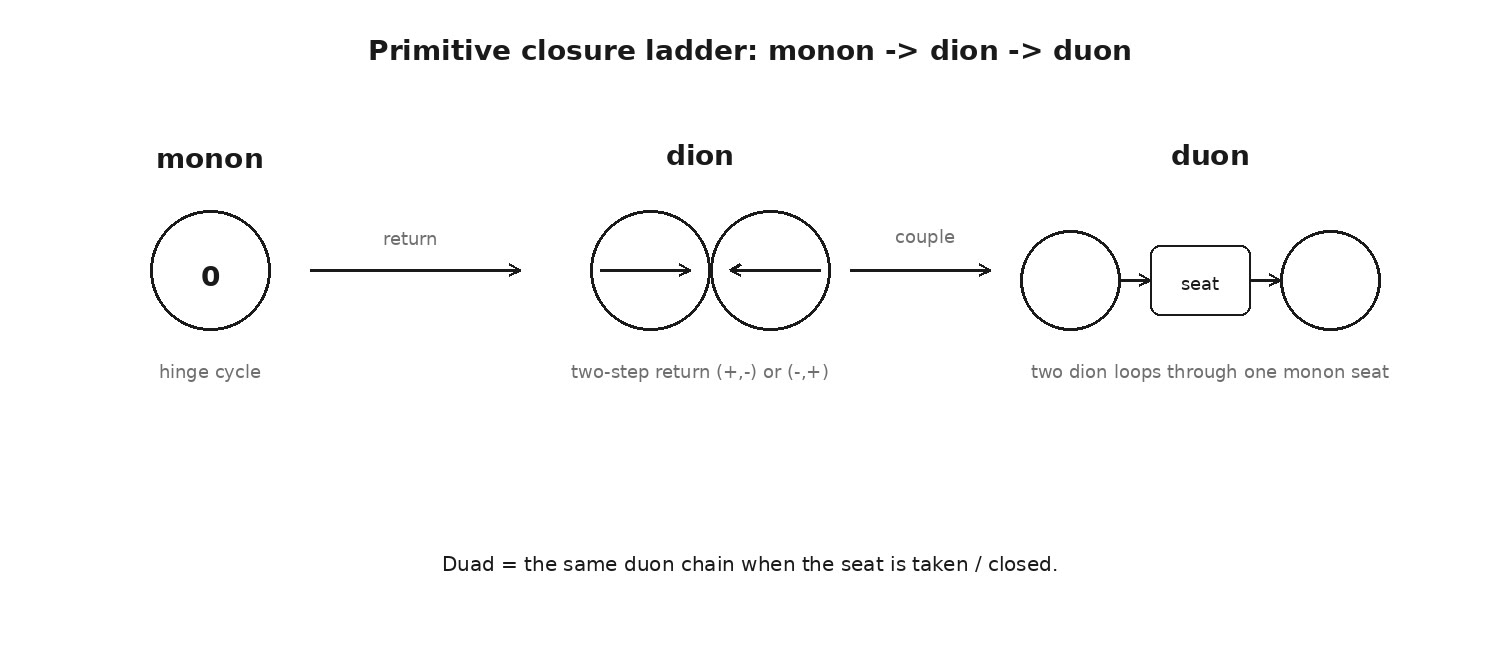
\includegraphics[width=0.82\linewidth]{figures_jpg/closure_ladder_monon_dion_duon.jpg}
\caption{Primitive closure ladder.}
\label{fig:closure-ladder}
\end{figure}

\aodprovenance{\eqnref{eq:cut-running-form},
\eqnref{eq:monon-cycle},
\eqnref{eq:duon-current},
\appref{app:curling-curls}.}
